\chapter{Scoring of Gestures}

\label{Chapter5_scoring} 

\begin{comment}
-------------------------------------------------
%								Chapter layout
5. Scoring of Gestures
	a. Angle Based Comparison Function
	b. Component Based Comparison Function
-------------------------------------------------
\end{comment}

%------------------------------------------------
%	SECTION 1 Angle Based Comparison Function
%------------------------------------------------
\section{Angle Based Comparison Function}
%description of algorithm and introduction to compare() function
This is the first way by which a hand gesture is scored. This scoring method compares one hand against another; namely, it is usually comparing the user's hand versus the target hand shown on the screen that the user was trying to imitate. It uses the angles between the three foremost bones, (distal, intermediate, proximal), of the five fingers as the primary means of determining how close a user's hand is to the target hand. It also uses the angle the wrist makes to the arm in its calculations to determine the final score for the hand. Figure \ref{fig:compare1} shows some important parts of the compare() function which scores the angular similarities between two hands. This function first makes sure that the two hands that are being compared are of the same kind; ie the hands must both be left or both must be right, otherwise the result of the compare() function will be 0. It then finds angles between adjacent finger bones in both hands and compares the two angles for the amount of similarity between them. This similarity between the two angles, which is the result of the compareAngles() method call, will be a number between 0 and 1. A weight applied to this similarity measure and then the result added to the summation variable x. This function relies on some weight parameters, see Figure \ref{fig:weights}, that are set higher for the longer bones that are closer to the knuckles. For example the proximal bones have a weight of 4; the intermediate bones have a weight of 2 and the distal bones have a weight of 1. This is because the bigger bones closer to the palm of the hand are a bit more limited in their mobility. Therefore, determining correlation between these corresponding bigger bones such as proximal has a higher influence on the overall value of the compare() function. 
\begin{figure}[H]
\centering
\begin{lstlisting}
public double compare(Hand h1, Hand h2) {
	//check if both hands are of the same type.
	if (h1.isLeft() == h2.isLeft()) {
		double x = 0;
		//wrist
		x += compareAngles(angleWristArm(h1), angleWristArm(h2))* weight_wrist;
		//five fingers "proximal". compareAngles always returns between 0-1
		x += compareAngles(anglePinkyProximal(h1), anglePinkyProximal(h2))*weight_pinky_proximal;
		x += compareAngles(angleRingProximal(h1), angleRingProximal(h2))* weight_ring_proximal;
		x += compareAngles(angleMiddleProximal(h1), angleMiddleProximal(h2))* weight_middle_proximal;
		x += compareAngles(angleIndexProximal(h1), angleIndexProximal(h2))* weight_index_proximal;
		x += compareAngles(angleThumbProximal(h1), angleThumbProximal(h2))* weight_thumb_proximal;
		//five fingers "intermediate"
		x += compareAngles(anglePinkyIntermediate(h1), anglePinkyIntermediate(h2))* weight_pinky_intermediate;
		...
		//five fingers "distal"
		x += compareAngles(anglePinkyDistal(h1), anglePinkyDistal(h2))* weight_pinky_distal;
		...
		x /= totalWeight();
		return x;
	} else{
		//if comparing left hand to right hand (or vice versa), return 0
		return 0; 
	}
}
\end{lstlisting}
\caption[Angular Comparison Function]{This snippet of code shows the main skeleton of the function that determines the similarity between two hands by comparing angles between various bones in the hands.}
\label{fig:compare1}
\end{figure}


\begin{figure}[H]
\centering
\begin{lstlisting}
//weights for various bone types 
static double weight_pinky_proximal = 4;
static double weight_pinky_intermediate = 2;
static double weight_pinky_distal = 1;
...
\end{lstlisting}
\caption[Bone Weights in Angular Comparison Function]{An example of the weights set for different bone types in the pinky finger.}
\label{fig:weights}
\end{figure}


%compareAngles() function
It is also worth looking into how the compareAngles() function is defined as this function determines what percentage of the weights get applied. It takes in two angles as it parameters. These angles are determined via various functions which find angles between consecutive bones of a specific finger. An example of one such function is shown in Figure \ref{fig:angleIndexDistal} which shows how the angle between the distal bone and the intermediate bone in the index finger is determined. The angle returned by these functions will always be less than 180 degrees because of the way the angleTo() function is defined in the Leap Motion API. 
\begin{figure}[H]
\centering
\begin{lstlisting}
private float angleIndexDistal(Hand h) {
	Vector direction1 = h.fingers().get(1).bone(Bone.Type.TYPE_DISTAL).direction();
	Vector direction2 = h.fingers().get(1).bone(Bone.Type.TYPE_INTERMEDIATE).direction();
	float rawAngle = direction1.angleTo(direction2);//always less than 180
	return normalize(rawAngle, h);//flips angle on xAxis if palm facing upwards
}
\end{lstlisting}
\caption[angleIndexDistal() Function]{This function is one example of how the angles between adjacent bones are determined.}
\label{fig:angleIndexDistal}
\end{figure}

The compareAngles() is a mathematical function that determines the similarity between two angles passed into it by using the cosine trigonometry function. It will return an number between 0 and 1. It first finds the difference between the two angels. If the angles are so far apart and the distance is greater than 45 degrees, then the function will return a zero to indicate that there is not any meaningful closeness between the two angles being compared. Figure \ref{fig:compareAngles} shows this function's code. 
\begin{figure}[H]
\centering
\begin{lstlisting}
private double compareAngles(float angle1, float angle2) {
	double differenceBtwAngles = Math.abs(angle1-angle2);
	//tmp can be at most pi/4 = 45
	double tmp = Math.min(differenceBtwAngles, Math.PI/4);
	//if tmp is exactly 45, will return 0. cos(90) = 0.
	return Math.cos(2*tmp);
}
\end{lstlisting}
\caption[compareAngles() Function]{This function determines how similar (or close together) two angles using cosine.}
\label{fig:compareAngles}
\end{figure}



	


%------------------------------------------------
%	SECTION 2 Component Based Comparison Function
%------------------------------------------------
\section{Component Based Comparison Function}
The second way by which a score is assigned to a hand representing an attempted gesture will be discussed in this section. 

%descripton of algorithm
The idea behind this method is to take a given hand and decompose it into smaller component that can be scored individually. Then these components scores will be combined to arrive at the cumulative score for the entire hand. Each finger is seen as a component. After considering all of the gestures being tested in this project, I realized that each finger can be in one of three main kinds of poses. All of the fingers except for the thumb are only seen in some variations of being straight, or being curved. The thumb, however, has its own special kind of pose, which deals with connecting to other fingers. For example in some of the gestures the thumb is touching the pinky; in some gestures it is touching the middle finger. Therefore, the third possible pose is represented by a finger name, such as "pinky" or "index" etc., and it represents the finger the thumb is touching in the gesture being analyzed. The way the algorithm is designed, it makes sense to assign this dynamic third pose to the thumb only. Figure \ref{fig:gestureComponents1} and Figure \ref{fig:gestureComponents2} shows one of the gestures used in this project, namely gesture9Left, to illustrate what is meant by the different poses different components of the hand can take. As we can see, all of the fingers are straight; the ring finger is curved; and the thumb is touching the ring finger. This "pose signature" of this gesture as it is used in code is shown in Figure \ref{fig:gesture9PoseSignature}. The pose signature for a certain gesture is the same regardless of whether left or right hand is being used. That is why the code sample shows two case statements for gesture9Left and gesture9Right. 

\begin{figure}[H]
    \centering
    \begin{minipage}{0.45\textwidth}
        \centering
        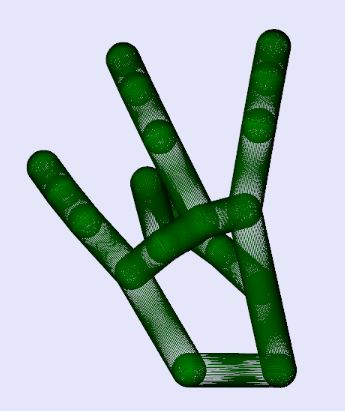
\includegraphics[scale=.5]{Figures/straight_curved_thumb1.JPG} % first figure itself
        \caption{Gesture showing different finger poses.}
		\label{fig:gestureComponents1}
    \end{minipage}\hfill
    \begin{minipage}{0.45\textwidth}
        \centering
        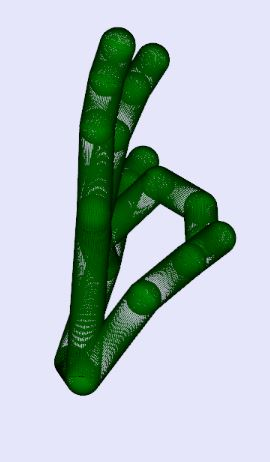
\includegraphics[scale=.5]{Figures/straight_curved_thumb2.JPG} % second figure itself
        \caption{Same gesture after a 90 degree rotation.}
        \label{fig:gestureComponents2}
    \end{minipage}
\end{figure}


\begin{figure}[H]
\centering
\begin{lstlisting}
case "gesture9Left":
case "gesture9Right":
	fingerPoseMap.put("index", "straight");
	fingerPoseMap.put("middle", "straight");
	fingerPoseMap.put("ring", "curved");
	fingerPoseMap.put("pinky", "straight");
	fingerPoseMap.put("thumb", "ring");
	break;
\end{lstlisting}
\caption[Finger Pose Mapping]{In the component based scroing, each gesture type gets a certain mapping for the kinds of poses fingers are expected to be in for that gesture.}
\label{fig:gesture9PoseSignature}
\end{figure}


% compare function and its helper functions
The comparison function for the component based scoring of hand gestures is shown in Figure \ref{fig:compare2}. It returns a number 0-100 just like the angle based comparison function to indicate the score for the hand being graded. This function gets the fingers for the hand and goes through and finds the individual grades for each finger. Then it combines the into a cumulative grade by weighing the fingers equally. 
\begin{figure}[H]
\centering
\begin{lstlisting}
public static int compare(Hand h, String gestureType) {
	FingerList fingerList = h.fingers();
	//make sure you have five fingers
	if (fingerList.count() == 5) {
		//calculate grades for each finger
		HashMap<String, Double> grades = getFingersGradedMap(getFingerHashMap(fingerList), getFingerPoseMap(gestureType));
		//grade for whole hand
		double totalGrade = cumulativeGrade(grades);
		//score 0-100
		return (int) (totalGrade * 100.0);
	}
	return -1;
}
\end{lstlisting}
\caption[Component Based Comparison Function]{}
\label{fig:compare2}
\end{figure}

To give a clearer idea about how the fingers actually get graded, the gradeFinger() function is shown in Figure \ref{fig:gradeFinger}. This function relies on three helper functions which calculate the straightness and curvedness of fingers and a function which returns the score for the thumb. 
\begin{figure}[H]
\centering
\begin{lstlisting}
private static double gradeFinger(HashMap<String, Finger> fingerMap, Finger f, String pose) {
	if (pose.equals("straight")) {
		return straightnessOfFinger(f);
	} else if (pose.equals("curved")) {
		return curvednessOfFinger(f);
	}
	//thumb is not touching any finger
	else if (pose.equals("thumb")) {
		return straightnessOfFinger(f);
	}
	//thumb touching other fingers
	else {
		Finger theFingerThumbTouches = fingerMap.get(pose);
		return getThumbScore(f, theFingerThumbTouches);
	}
}
\end{lstlisting}
\caption[gradeFinger() Function]{Given a finger a certain pose, this function returns a grade (0-1) for that finger. It uses helper functions to calculate grades for a finger in one the three main kinds of poses.}
\label{fig:gradeFinger}
\end{figure}		

Two of these helper functions, the straightnessOfFinger() and curvednessOfFinger() are shown in Figure \ref{fig:straightCurvedHelperFunctions}. These functions first find the sum of the angle between consecutive bones in the finger that is being graded. For a perfectly straight finger, the sum of these angles should be around 0 degrees. However, to allow for some leniency in the grading 30 degrees are subtracted from the sum of the angles. This allows for a buffer for the user that we intuitively as humans might guage as being relatively straight. For measuring the curvedness of a finger, the sum of the angles between the bones of the fingers should be as close to 270 as possible. However, again a buffer was provided to allow for not perfectly curled fingers to still be valid enough to return a good score.Of course these parameters can be adjusted if this application was used in the real world. These were what I felt were good parameters when I wrote these grading functions.
\begin{figure}[H]
\centering
\begin{lstlisting}
private static double straightnessOfFinger(Finger f) {
	//best case = 0; worst case is: 90+90+90 = 270.
	double sumOfAngles = getSumOfThreeAnglesBetweenFingerBones(f);
	sumOfAngles = sumOfAngles - 30;//offset by 30 degrees
	double score = sumOfAngles / 270;//closer to 0 means a better score
	score = 1 - score;//conventional scale: 0 = bad, 1 = good.
	return snapScore0to1(score);
}
private static double curvednessOfFinger(Finger f) {
	//best case is: 90+90+90 = 270; adjusted bestcase = 210; worst case = 0;
	double sumOfAngles = getSumOfThreeAnglesBetweenFingerBones(f);
	double score = sumOfAngles / 210;//closer to 1 means a better score
	return snapScore0to1(score);
}
\end{lstlisting}
\caption[straightnessOfFinger() and curvednessOfFinger()]{These helper functions are similar to each other. They are used in grading the four fingers.}
\label{fig:straightCurvedHelperFunctions}
\end{figure}		

The helper function getThumbScore(), shown in Figure \ref{fig:getThumbScore} is the more complicated of the three. The way a score is calculated for a thumb is by finding the distance between the tip bone of the thumb and any of the three outermost bones on the finger the thumb is supposed to be touching. The smallest distance is chosen as the tip of the thumb might be closer to any three of the distal, intermediate or proximal bones. This is because some people rest their thumb on the tip of the distal bone, others rest on top of the distal or the intermediate. This distance is scaled down by the smallest bone length multiplied by a scaling factor. Like the other two functions, straightnessOfFinger() and curvednessOfFinger(), the score that is returned is snapped to be between 0-1. 
\begin{figure}[H]
\centering
\begin{lstlisting}
private static double getThumbScore(Finger thumb, Finger otherFinger) {
	//bones in thumb and finger
	HashMap<String, Bone> thumbMap = getHashMapOfBonesFromFinger(thumb);
	HashMap<String, Bone> fingerMap = getHashMapOfBonesFromFinger(otherFinger);
	//get center point of thumb's tip bone
	Vector thumbTip = thumbMap.get("distal").center();
	//finger bones
	Bone d = fingerMap.get("distal");
	Bone i = fingerMap.get("intermediate");
	Bone p = fingerMap.get("proximal");
	//length of bones
	float smallestBoneLength = (Math.min(Math.min(d.length(), i.length()), p.length()));
	//distances from thumb tip to finger bones
	float d1 = thumbTip.distanceTo(d.center());
	float d2 = thumbTip.distanceTo(i.center());
	float d3 = thumbTip.distanceTo(p.center());
	double minDistance = (double) (Math.min(Math.min(d1, d2), d3));
	//scale and score
	double distanceScaledByBoneLength = minDistance / (smallestBoneLength * 3);
	double score = 1 - distanceScaledByBoneLength;
	return snapScore0to1(score);
}
\end{lstlisting}
\caption[getThumbScore() Helper Function]{This function calculates the grade for the thumb that is supposed to be touching one of the four fingers. It calculates this score by distances rather than using angles.}
\label{fig:getThumbScore}
\end{figure}

%doenst need a target hand to compare against. explain why this is good. 
One final thing to note about this comparison function is that it does not rely on a target hand for the comparison. Instead it relies on set gesture poses that are expected for the different gestures to arrive at its score. Therefore, it is more stable form of comparison. If the target hands are themselves not very good examples of the gestures being displayed, the angle based comparison method's performance could be unnecessarily affected. 
